\documentclass[10pt, compress]{beamer}

\usetheme{m}

\usepackage{booktabs}
\usepackage[scale=2]{ccicons}
\usepackage{minted}
\usepackage{wrapfig}
\usepackage[font={footnotesize}]{caption}

\usepgfplotslibrary{dateplot}

\usemintedstyle{trac}

\title{Go Aber - Fitness Tracking Application}
\subtitle{\small{SEM5640 - Developing Advanced Internet-Based Applications}}
%\date{\today}
\author{\footnotesize{Connor Goddard (clg11), Samuel Jackson (slj11), Helen Harman (heh14), Daniel McGuckin (dam34), Craig Heptinstall (crh13)}}
\institute{Aberystwyth University}

\begin{document}

\maketitle

\begin{frame}[fragile]
  \frametitle{Introduction}
  
  \small {
  
    Project: Develop an application that acquires activity data from 3rd party sources and keep users engaged through challenges and progress updates
    
    \vspace{10pt}
    
    Two systems produced: One Java EE, One .NET
    
    }

\end{frame}

\begin{frame}[fragile]
  \frametitle{Overview}
  
  \small{
  
  	\begin{itemize}
    	\item Project Status
    	\item Methodology
    	\item Design
    	\item Implementation \& Issues
    	\item Live Demo
    	\item Evaluation \& Conclusions
    \end{itemize}
    
    }

\end{frame}

\plain{Project Status}

\begin{frame}[fragile]
\frametitle{Project status}

\begin{itemize}
	\item Majority of requirements completed, with a small number of exceptions
		\begin{itemize}
			\item Fitbit connectivity in JavaEE
			\item Email sending from application
		\end{itemize}
	\item Application tests
		\begin{itemize}
			\item User testing – Interoperability notable
			\item Mocks and unit tests
			\item Cucumber
		\end{itemize}
\end{itemize}
\end{frame}

\plain{Design}

\begin{frame}[fragile]
  \frametitle{Design}
  
   \small{ 
   	
   		From requirements analysis we a couple of areas where we felt needed to be discussed in more depth.
   		
   		\begin{itemize}
			\item Conceptual system architecture
   			\item Entity relationship diagram
   		\end{itemize}
     
   }

\end{frame}

\begin{frame}[fragile]
  \frametitle{Design - Architecture}
  
   \small{
   	 Key points:

     \begin{itemize}
     	\item Our first thoughts on a very high level conceptual overview of the system.
   		\item Should be essentially the same for both. Technology specific decisions left to developer.
   		\item Three distinct client facing parts.
   		\item Business logic deliberately left vague.
   	  \end{itemize}
   	  
   	  \begin{wrapfigure}{r}{0.40\textwidth}
	  \begin{center}
      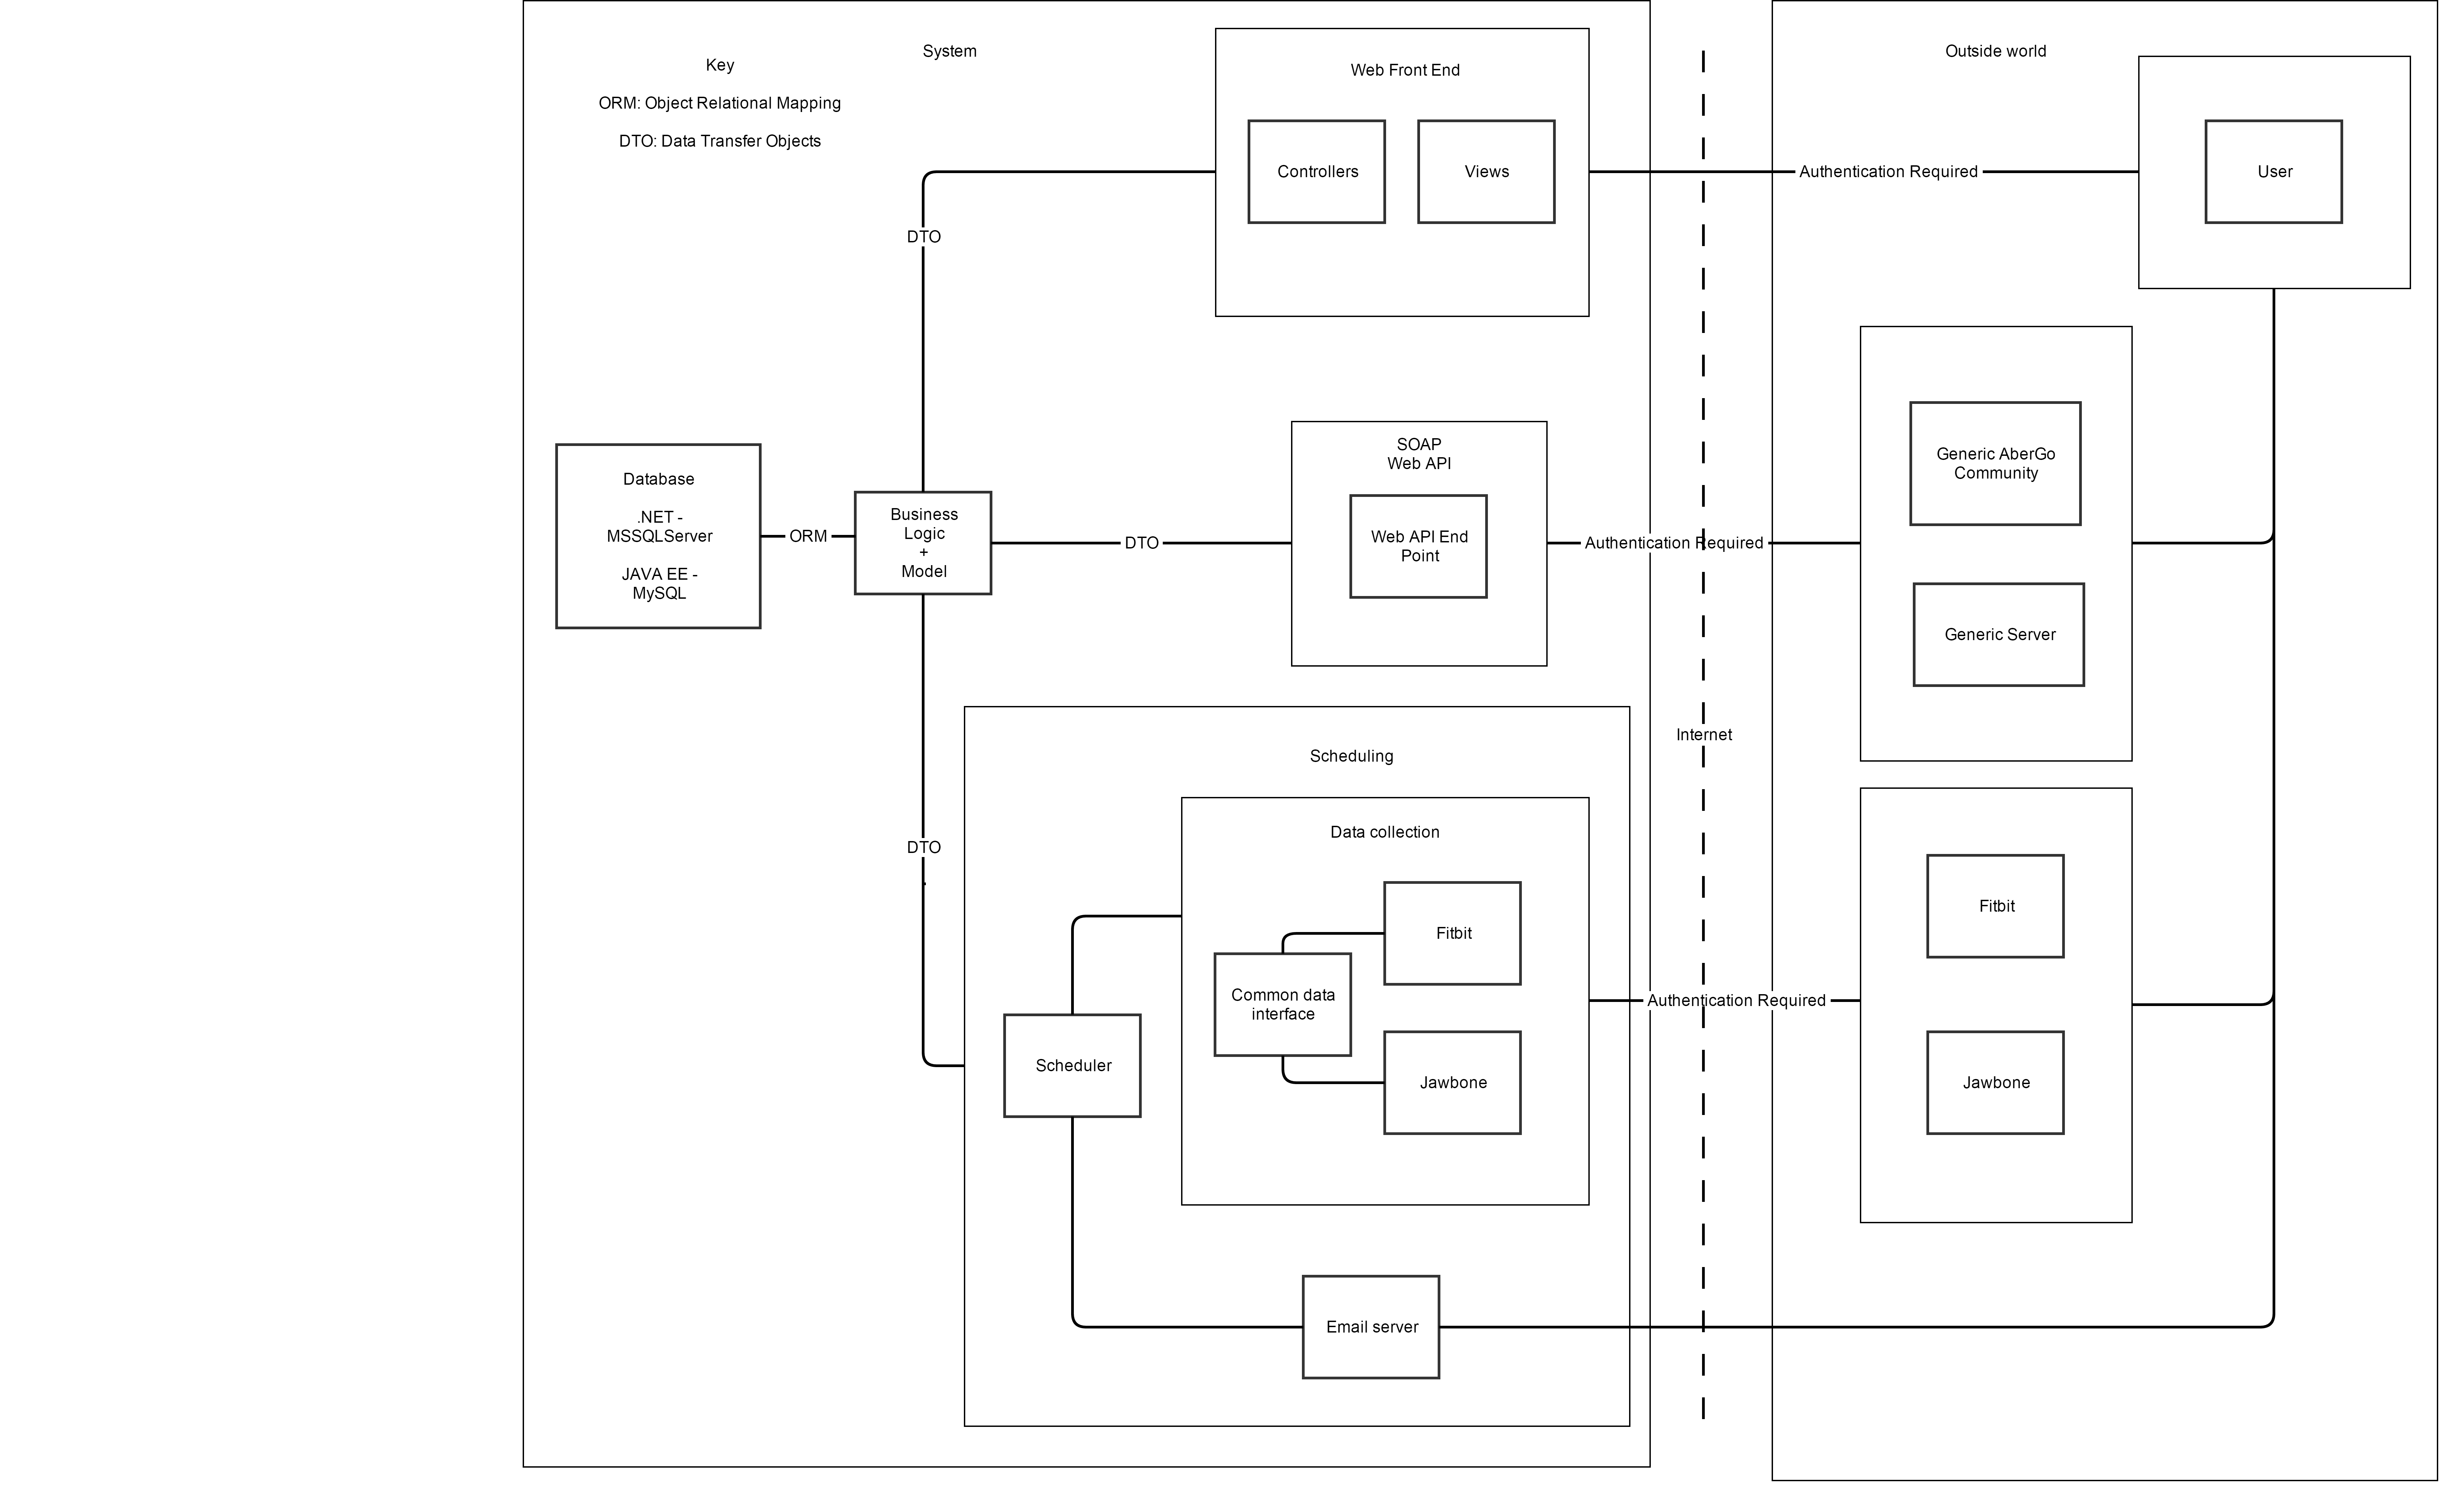
\includegraphics[width=1.0\textwidth]{../design/system/groupproject_systemarchitecture.png}
	  \end{center}
	  \end{wrapfigure}
   }

\end{frame}

\begin{frame}[fragile]
  \frametitle{Design - ERD}
  
  
    	   \begin{wrapfigure}{r}{0.6\textwidth}
%   \vspace{-15pt}
  \begin{center}
    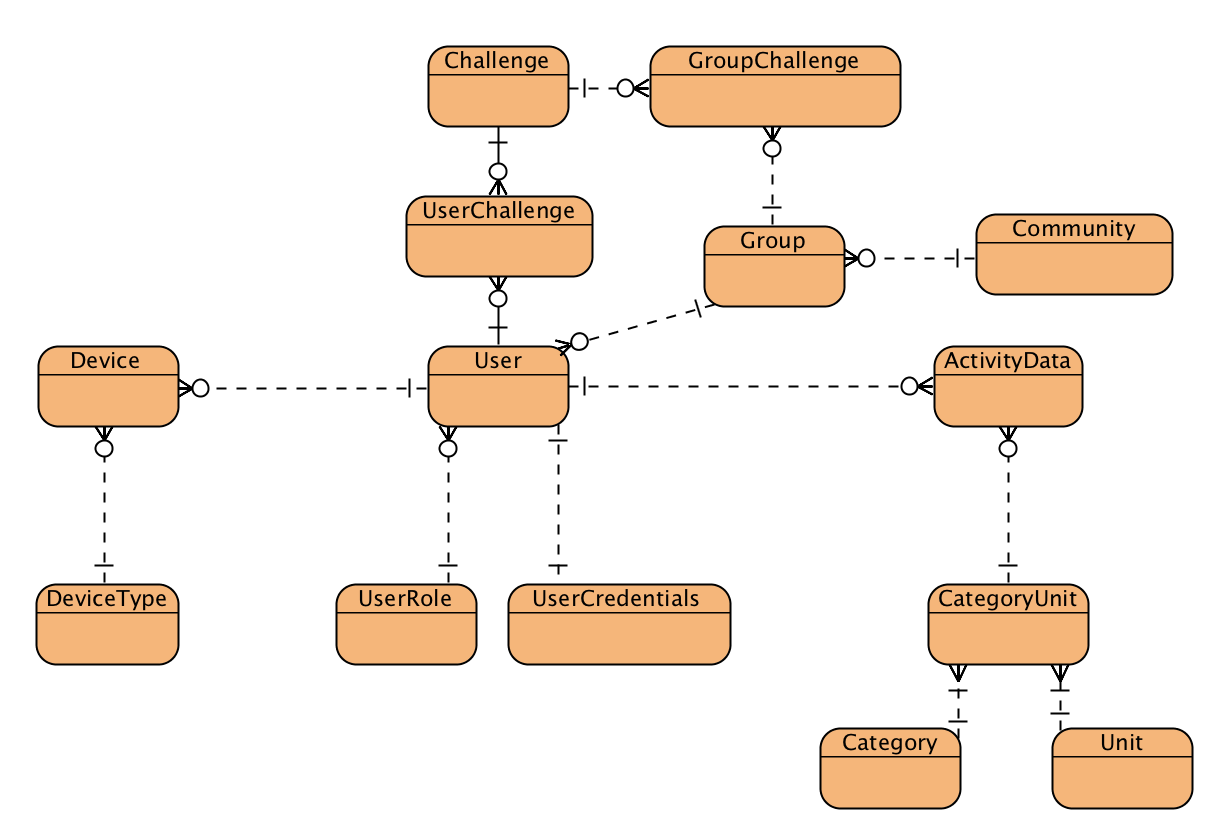
\includegraphics[width=0.6\textwidth]{../design/database/GoAber-ERD.png}
  \end{center}
  \end{wrapfigure}
  
  	Key Points:
  
  	\begin{itemize}
		\item Artefact from our first discussion a bout the database model
	   	\item Activity data: One table for all types, one row per entry
	   	\item User can only have one row
	   	\item Our data model very closely mimicked this.
	\end{itemize}
     
%   \small{
%   	  \begin{wrapfigure}{r}{1.0\textwidth}
%	  \begin{center}
%      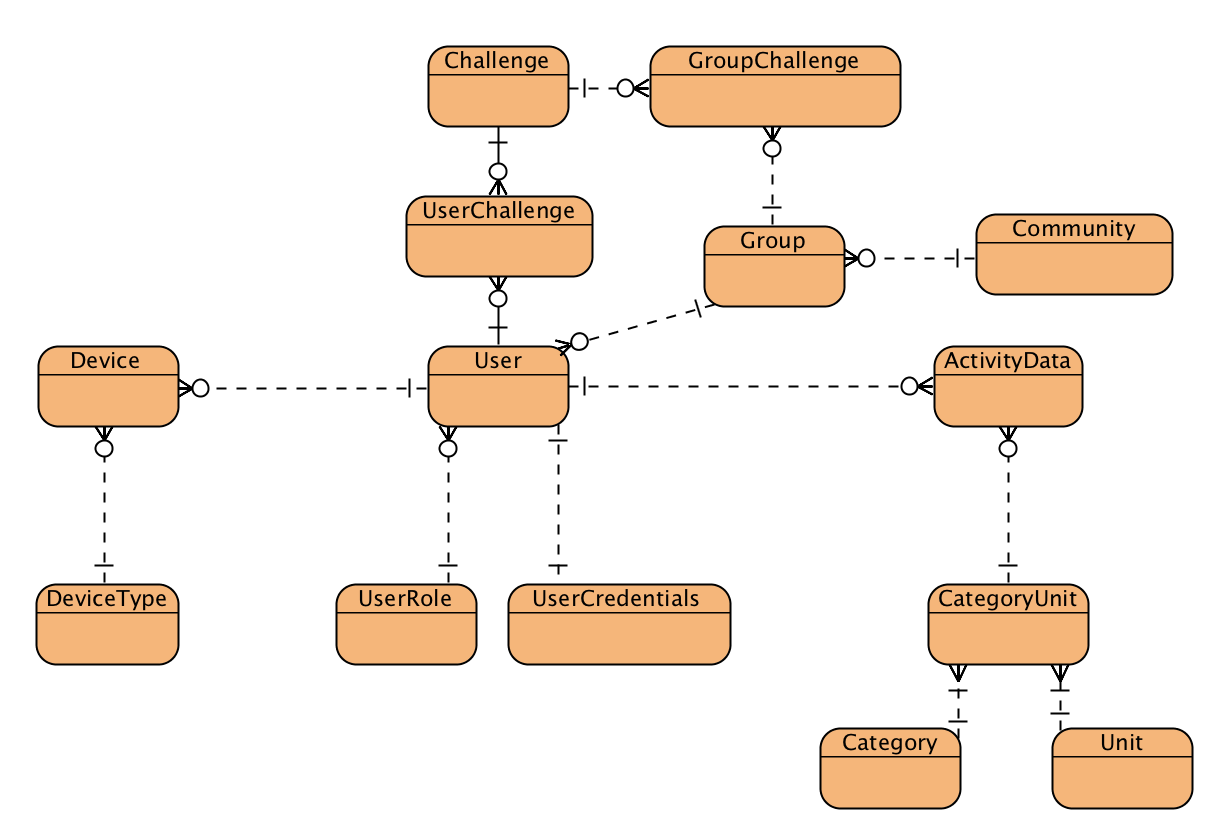
\includegraphics[width=1.0\textwidth]{../design/database/GoAber-ERD.png}
%	  \end{center}
%	  \end{wrapfigure}
%   }

\end{frame}


\plain{Project Management}

\begin{frame}[fragile]
  \frametitle{Project Characteristics}
  
  \vspace{-10pt}
  
   \small{ 
  		
  		\begin{enumerate}
  		
  			\item \textbf{Team Resources}
  			
  			\begin{itemize}
  			\footnotesize{
  			\item All members expected to hold development responsibilities.
  			\item Delegation of tasks manageable at the scale of an \textit{individual developer}. 
  			\item Multiple allocation of roles required (between technical and organisational aspects).
  			}
  			
  			\end{itemize}
  			
  			
  			\item \textbf{Technical Complexity}
  		
  			\begin{itemize}
  			\footnotesize{
%  			\item Non-trivial size \& complexity.
  			\item Lack of prior team knowledge and experience in primary technologies (ASP.NET \& JavaEE).
  			\item Expectation to face technical challenges and need for design review.
  			\item Required flexibility with respect to work (re-)scheduling and design changes.
  			\item Too much up-front design likely to be in vain.
  			\item Deployment of enhanced individual developer skill-sets to appropriate technical areas. 
  			}
  			\end{itemize}
  			
  			\item \textbf{Project Budget}
  		
  			\begin{itemize}
  			\footnotesize{
  			\item Time represented the primary budget constraint for the project.
  			\item Prioritisation of work to be crucial given expected technical complexity.
  			\item No particular expectation for customer-led requirements changes, but important to provide some buffer for this.
  			}
  			\end{itemize}
  			
  			
  		\end{enumerate}
  	
     }

\end{frame}

\begin{frame}[fragile]
  \frametitle{Development Methodology}
  
   \small{ 
   
   \textbf{SCRUM} selected as the primary development methodology.
   
   Iterative approach to development deemed most appropriate given team's lack of prior experience.
   
	% Iterative approach mitigated teams lack of experience.
	
		\begin{itemize}
  			\footnotesize{
  			\item Provided \textit{regular} opportunities to re-evaluate work priorities, and to discuss technical issues as a team.
			\item Flexibility to re-visit the design in light of technical constraints or new-found developer knowledge/research.
  			}
  		\end{itemize}
  		
  	Up-front planning of work allowed for clear visibility in terms of task ownership and bug management.
  	
  	SCRUM does not enforce a fixed set of development practices. \textit{This allowed for flexibility with respect to testing, design \& refactoring}.  
  	
  	
	  
   }
   
\end{frame}

\begin{frame}[fragile]
  \frametitle{Development Approach}
  
   \small{ 
   
   \textbf{Work Planning}
   
   \begin{itemize}
  			\footnotesize{
  			\item 6-day Sprint cycles (12-day for first sprint).
  			\item Weekly \textbf{sprint retrospective} and \textbf{sprint planning} meetings. - In collaboration with project manager (Nigel) 
  			\item No daily-stand up meeting (\textit{flexbility to do this!})
%  			\item Product backlog managed by dedicated Product Owner - responsible for prioritising work left to accomplish across the remaining project duration.
%  			\item Development team (which included the PO) decided on how much work could be accomplished per sprint, and how many sprints would be required.
%  			\item Final sprint defined as ``spare" in preparation for overdue work.
  			}
  		\end{itemize}
  		  		
  		
  	\textbf{Progress Monitoring}
   
   \begin{itemize}
  			\footnotesize{
  			\item Developers required to estimate remaining work for allocated tasks.
  			\item Estimates collated into a \textbf{burn-down chart} for the current sprint.  
			\item Team velocity provided general indication as to the overall performance with respect to accomplishing committed tasks.
  			}
  		\end{itemize}
  		
  \textbf{Development}
   
   \begin{itemize}
  			\footnotesize{
  			\item Continuous integration.
  			\item Use of \textit{Git-flow} branching model.
  			\item All individual development work undertaken in both JavaEE \& ASP.NET. 
  			}
  			
  		\end{itemize}
  			  
   }
   
\end{frame}


\begin{frame}[fragile]
  \frametitle{Development Approach}
  
   \small{ 
   
       	 \textbf{Design}
   
   \begin{itemize}
  			\footnotesize{
  			\item Attempted to adopt an \textbf{evolutionary design} approach.
  			\item Team had scope to address issues at a \textit{design level}, rather than been forced to make ``ad-hoc" changes/fixes at an implementation level.
  			\item Weekly SCRUM meetings complemented this approach, providing regular opportunities to re-visit the design \textit{all together as a team}.
  			}
  		\end{itemize}
  		
   \textbf{Testing}
   
   \begin{itemize}
  			\footnotesize{
  			\item No ``official" testing strategy was adopted, however aspects from both TDD and BDD were utilised (e.g. Acceptance testing and regular re-factoring).
  			\item Two ``levels" of testing:
  			
  			\begin{enumerate}
  			\footnotesize{
  				\item \textbf{Unit \& Regression Testing} - Undertaken by  component author. \textbf{Included the use of mocked test doubles.}
  				\item \textbf{Acceptance Testing} - Undertaken either: manually as part of integration process; or automatically via Cucumber framework.
  				}
  			\end{enumerate}
  			
  				}
  		\end{itemize}
  		

   }
   
\end{frame}

\begin{frame}[fragile]
  \frametitle{Visual Studio Online}
  
   \small{ 
   	
   	Suite of web-based tools designed to support development teams wishing to deliver software using an agile approach.
   	
   	Free for teams with up to five developers.
   	
   	Included a comprehensive range of facilities, including:
   	
   	  \begin{itemize}
  			\footnotesize{
  			\item Interactive Kanban-style work planning boards
  			\item Automatic tracking and presentation of project metrics (inc. velocity, burn-down and cumulative flow)
  			\item Integrated Git-based version control system
  			\item Integrated build server \& automated testing environment (Continuous Integration)
  			}
  		\end{itemize}
   	
   }
   
\end{frame}

\begin{frame}[fragile]
  \frametitle{Team Performance}
  

   
    \begin{columns}[T,onlytextwidth]
    \hspace*{-10pt}
    \column{0.48\textwidth}
    
	   	\begin{center}
   
\begin{figure}[!ht]
  \centering
  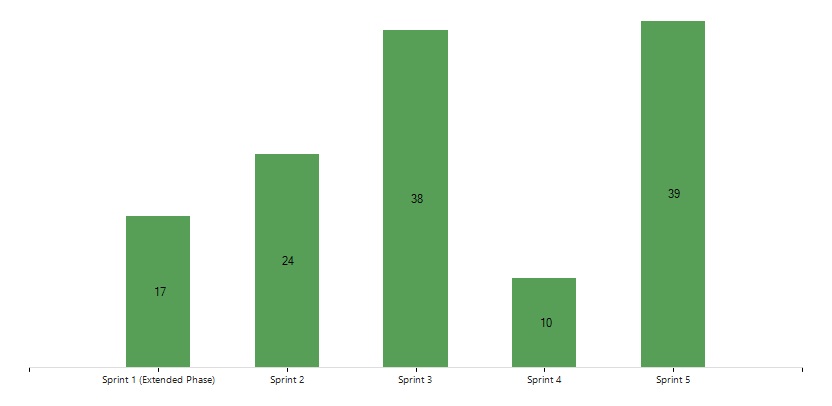
\includegraphics[width=1.1\textwidth]{Velocity.png}
  \caption{Team velocity performance over project duration.}
\end{figure}

  \end{center}

    \column{0.48\textwidth}
 \begin{center}
\begin{figure}[!ht]
  \centering
  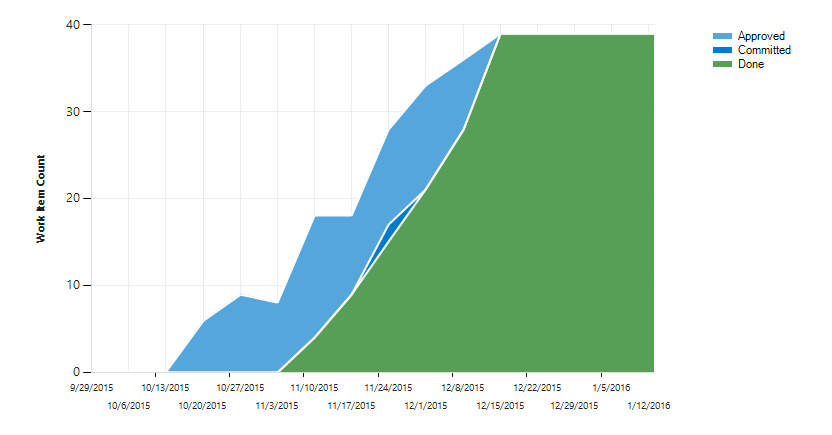
\includegraphics[width=1.1\textwidth]{CumulativeFlow.png}
  \caption{Cumulative flow of features over project duration.}
\end{figure}
  \end{center}

  \end{columns}
   
\end{frame}


\plain{Implementation}

\begin{frame}[fragile]
  \frametitle{Implementation}
  
   \small{ 
   
    \begin{table}
    
    \begin{tabular}{r p{2.8cm} p{2.5cm}}
%      \toprule
      & \multicolumn{1}{ c }{JavaEE} & \multicolumn{1}{ c }{ASP.NET}\\
%      \midrule
		\cline{2-3}
      \multicolumn{1}{ r| }{Authentication} & JDBC Realm & Identity Framework\\
      \multicolumn{1}{ r| }{ORM} & JPA (EclipseLink) & Entity Framework (Code First) \\
      \multicolumn{1}{ r| }{Scheduling} & Managed Execution Schedular & Hangfire Library \\
      \multicolumn{1}{ r| }{UI} & Primefaces Library & ASP.NET Razor \\
%      \bottomrule
    \end{tabular}
    \caption{Key technology choices between JavaEE \& ASP.NET platforms.}
  \end{table}
  	  
   }
   
\end{frame}
  
  \begin{frame}[fragile]
  \frametitle{Implementation}
  
   \small{ 
   
   \textbf{Key Issues:}
   
   \begin{enumerate}
  			
  	 \item JavaEE Realms
  	 
     \begin{itemize}
  			\footnotesize{
  			\item Lack of clear vendor documentation. 
  			\item Resorted to following tutorials created by previous affected developers.
  			\item Glassfish configuration (\url{asadmin} tool for scripting) 
  			}
  	 \end{itemize}
  	 
  	 \item Change of RDBMS
  	 
     \begin{itemize}
  			\footnotesize{
  			\item Originally chose to use MySQL - common between both platforms.
  			\item Switched to using SQL Server for ASP.NET - default support by Identity Framework.
  			\item Caused unintended delays due to the need to revise the database structure.
  			}
  	 \end{itemize}
  	 
  	 \item Multi-tier Architecture
  	 
     \begin{itemize}
  			\footnotesize{
  			\item Application design could have been improved to better support a multi-tier architecture.
  			\item Significant proportion of business logic residing in controller classes or service classes organised in WAR.
  			\item Partial support for Service Layer pattern (via dedicated service classes).
  			}
  	 \end{itemize}
  		
  				
  			\end{enumerate}
  			
  	  
   }
   
\end{frame}

%\begin{frame}[fragile]
%  \frametitle{Militarised AI \& Automated Weapons}
%  
%   \small{ 
%   
%   	\textbf{Literature:} ``Comment: Ethics of Artificial Intelligence" (Article), Stuart Russell, Nature (2015)
%   	
%   	\vspace{10pt}
%   	
%   	Historically, military organisations have always been positioned at the forefront of technological advancement. - With AI, this is no different.
%   	
%%   	Idea of machines taking on decisions over life and death do not sit well with many people.
%   	
%   		       \begin{wrapfigure}{r}{0.40\textwidth}
%  \begin{center}
%  \vspace{-15pt}
%    \includegraphics[width=0.35\textwidth]{code_darpa.jpg}
%    \vspace{-20pt}
%  \end{center}
%  \end{wrapfigure}
%   	
%   	Author argues that all the `components' needed for LAWS already exist - ``\textit{they just need to be combined}" (FLA and CODE DARPA projects).
%   	
%   Mapping jurisdiction of existing humanitarian laws to the actions of autonomous weapons. - Gaps in applicability due to subjective reasoning.
%   
%   Need for the AI community to take a position on acceptable use of their technology.
%   
%     }

%\end{frame}

\plain{Demonstration}


\begin{frame}[fragile]
\frametitle{Evaluation}

\begin{itemize}
	\item Starting development
		\begin{itemize}
			\item Key concerns and questions addressed
			\item Setting up development machines was time consuming, including a database change
		\end{itemize}
	\item During development and testing
		\begin{itemize}
			\item Use of TFS was hugely useful during sprints
			\item Tests were created, though more could have been done, and more efficiently
		\end{itemize}
	\item Team collaborated successfully, and put in an even amount of effort from the requirements stage through to the documentation and demonstration stage of the project
\end{itemize}
\end{frame}

\begin{frame}[fragile]
  \frametitle{Conclusions}
  
  	\begin{itemize}
		\item Produced two working applications
		\item Followed methodology \& improved as we went along
		\item Major issues were time, testing, and lack of experience with technology.
	\end{itemize}

\end{frame}


\plain{Any Questions? \\ \vspace{0.2cm} \footnotesize{Slide Design: Matthias Vogelgesang - (\href{https://github.com/matze/mtheme}{Github})}}

\end{document}
